\chapter{Computational Thinking}
\label{chap:computational-thinking}

\section{Decomposition}
To manage the complexity of this multi-faceted system, we applied the principle of \textbf{Decomposition} to break the application down into six distinct, manageable modules. This modular architecture allows for parallel development and easier debugging.

% --- HIGH-LEVEL SYSTEM OVERVIEW ---
\begin{figure}[H]
\centering
\begin{forest}
    for tree={
        grow=east,
        parent anchor=east,
        child anchor=west,
        forked edge,
        edge={-Latex, thick, draw=black!60},
        l sep=2.5cm,
        s sep=0.8cm,
        align=center,
        font=\sffamily,
        shape=rectangle,
        rounded corners=4pt,
        draw=black!50,
        line width=0.5pt,
        inner sep=8pt,
        drop shadow,
    },
    where level=0{font=\sffamily\bfseries\large, line width=1pt}{},
    where level=1{font=\sffamily\bfseries}{},
    [{\textbf{Tourism System}\\Ho Chi Minh City}, fill=red!20
        [{\textbf{1. Data Acquisition}\\Module}, fill=blue!15]
        [{\textbf{2. AI/ML Module}}, fill=purple!15]
        [{\textbf{3. Routing Engine}}, fill=orange!15]
        [{\textbf{4. Safety/SOS Module}}, fill=green!15]
        [{\textbf{5. Backend API}}, fill=cyan!15]
        [{\textbf{6. Frontend UI}}, fill=yellow!20]
    ]
\end{forest}
\caption{System Decomposition Overview}
\label{fig:decomposition-overview}
\end{figure}

The following figures detail the sub-components of each module:

% --- MODULE 1 & 2: Data Acquisition + AI/ML ---
\begin{figure}[H]
\centering
\begin{minipage}[t]{0.48\textwidth}
\centering
\begin{forest}
    for tree={
        grow=east,
        parent anchor=east,
        child anchor=west,
        forked edge,
        edge={-Latex, thick, draw=black!60},
        l sep=1.2cm,
        s sep=0.5cm,
        align=center,
        font=\sffamily\small,
        shape=rectangle,
        rounded corners=3pt,
        draw=black!50,
        line width=0.5pt,
        inner sep=5pt,
        drop shadow,
    },
    where level=0{font=\sffamily\bfseries}{},
    [{\textbf{Data Acquisition}\\Module}, fill=blue!15
        [{Camera Crawler}, fill=blue!8]
        [{Bus Data ETL}, fill=blue!8]
        [{POI Scraper}, fill=blue!8]
    ]
\end{forest}
\subcaption{Data Acquisition Module}
\end{minipage}%
\hfill
\begin{minipage}[t]{0.48\textwidth}
\centering
\begin{forest}
    for tree={
        grow=east,
        parent anchor=east,
        child anchor=west,
        forked edge,
        edge={-Latex, thick, draw=black!60},
        l sep=1.2cm,
        s sep=0.5cm,
        align=center,
        font=\sffamily\small,
        shape=rectangle,
        rounded corners=3pt,
        draw=black!50,
        line width=0.5pt,
        inner sep=5pt,
        drop shadow,
    },
    where level=0{font=\sffamily\bfseries}{},
    [{\textbf{AI/ML Module}}, fill=purple!15
        [{YOLO Detection}, fill=purple!8]
        [{LLM Planner}, fill=purple!8]
        [{Fuzzy Matching}, fill=purple!8]
        [{Congestion Model}, fill=purple!8]
    ]
\end{forest}
\subcaption{AI/ML Module}
\end{minipage}
\caption{Decomposition of Data Acquisition and AI/ML Modules.}
\label{fig:decomposition-data-ai}
\end{figure}

% --- MODULE 3 & 4: Routing Engine + Safety/SOS ---
\begin{figure}[H]
\centering
\begin{minipage}[t]{0.48\textwidth}
\centering
\begin{forest}
    for tree={
        grow=east,
        parent anchor=east,
        child anchor=west,
        forked edge,
        edge={-Latex, thick, draw=black!60},
        l sep=1.2cm,
        s sep=0.5cm,
        align=center,
        font=\sffamily\small,
        shape=rectangle,
        rounded corners=3pt,
        draw=black!50,
        line width=0.5pt,
        inner sep=5pt,
        drop shadow,
    },
    where level=0{font=\sffamily\bfseries}{},
    [{\textbf{Routing Engine}}, fill=orange!15
        [{Graph Builder}, fill=orange!8]
        [{A* Pathfinding}, fill=orange!8]
        [{TomTom Proxy}, fill=orange!8]
        [{Route History}, fill=orange!8]
    ]
\end{forest}
\subcaption{Routing Engine}
\end{minipage}%
\hfill
\begin{minipage}[t]{0.48\textwidth}
\centering
\begin{forest}
    for tree={
        grow=east,
        parent anchor=east,
        child anchor=west,
        forked edge,
        edge={-Latex, thick, draw=black!60},
        l sep=1.2cm,
        s sep=0.5cm,
        align=center,
        font=\sffamily\small,
        shape=rectangle,
        rounded corners=3pt,
        draw=black!50,
        line width=0.5pt,
        inner sep=5pt,
        drop shadow,
    },
    where level=0{font=\sffamily\bfseries}{},
    [{\textbf{Safety/SOS Module}}, fill=green!15
        [{Report SOS}, fill=green!8]
        [{List Alerts}, fill=green!8]
        [{Map Markers}, fill=green!8]
    ]
\end{forest}
\subcaption{Safety/SOS Module}
\end{minipage}
\caption{Decomposition of Routing Engine and Safety/SOS Modules.}
\label{fig:decomposition-routing-sos}
\end{figure}

% --- MODULE 5 & 6: Backend API + Frontend UI ---
\begin{figure}[H]
\centering
\begin{minipage}[t]{0.48\textwidth}
\centering
\begin{forest}
    for tree={
        grow=east,
        parent anchor=east,
        child anchor=west,
        forked edge,
        edge={-Latex, thick, draw=black!60},
        l sep=1.2cm,
        s sep=0.5cm,
        align=center,
        font=\sffamily\small,
        shape=rectangle,
        rounded corners=3pt,
        draw=black!50,
        line width=0.5pt,
        inner sep=5pt,
        drop shadow,
    },
    where level=0{font=\sffamily\bfseries}{},
    [{\textbf{Backend API}}, fill=cyan!15
        [{Auth Endpoints}, fill=cyan!8]
        [{Routing API}, fill=cyan!8]
        [{Camera API}, fill=cyan!8]
        [{SOS API}, fill=cyan!8]
    ]
\end{forest}
\subcaption{Backend API}
\end{minipage}%
\hfill
\begin{minipage}[t]{0.48\textwidth}
\centering
\begin{forest}
    for tree={
        grow=east,
        parent anchor=east,
        child anchor=west,
        forked edge,
        edge={-Latex, thick, draw=black!60},
        l sep=1.2cm,
        s sep=0.5cm,
        align=center,
        font=\sffamily\small,
        shape=rectangle,
        rounded corners=3pt,
        draw=black!50,
        line width=0.5pt,
        inner sep=5pt,
        drop shadow,
    },
    where level=0{font=\sffamily\bfseries}{},
    [{\textbf{Frontend UI}}, fill=yellow!20
        [{Map Components}, fill=yellow!10]
        [{Route Display}, fill=yellow!10]
        [{Congestion Overlay}, fill=yellow!10]
        [{User Dashboard}, fill=yellow!10]
    ]
\end{forest}
\subcaption{Frontend UI}
\end{minipage}
\caption{Decomposition of Backend API and Frontend UI Modules.}
\label{fig:decomposition-backend-frontend}
\end{figure}

% % --- SYSTEM ARCHITECTURE DIAGRAM ---
% \begin{figure}[H]
% \centering
% \begin{tikzpicture}[node distance=2cm]
%     \tikzset{arrow/.style={->, thick}}
%     \tikzset{
%         process/.style={rectangle, minimum width=3.8cm, minimum height=1.2cm, draw=black, align=center},
%         io/.style={trapezium, trapezium left angle=70, trapezium right angle=110, minimum width=3.8cm, minimum height=1.2cm, draw=black, align=center}
%     }
%     % Nodes
%     \node (data) [process, fill=blue!20] {Data Acquisition\\(Cameras/Bus/POI)};
%     \node (ai) [process, fill=purple!20, right=of data, xshift=1cm] {AI Module\\(YOLO Detection + LLM)};
%     \node (db) [process, fill=gray!20, below=of data] {Central Database\\(SQLite/JSON)};
%     \node (routing) [process, fill=orange!20, below=of ai] {Routing Engine\\(A* Pathfinding)};
%     \node (api) [process, fill=cyan!20, below=of routing, xshift=-2.5cm] {Flask REST API\\(Backend)};
%     \node (web) [io, below=of api, align=center] {Web Interface\\(Folium/HTML)};

%     % Arrows
%     \draw [arrow] (data) -- node[above, font=\footnotesize] {Raw Feeds} (ai);
%     \draw [arrow] (data) -- node[left, font=\footnotesize] {Static Data} (db);
%     \draw [arrow] (ai) -- node[right, font=\footnotesize] {Inferences} (db);
%     \draw [arrow] (db) -- node[above, font=\footnotesize] {Graph Data} (routing);
%     \draw [arrow] (db) -- node[below left, font=\footnotesize] {JSON} (api);
%     \draw [arrow] (routing) -- node[right, font=\footnotesize] {Optimal Path} (api);
%     \draw [arrow] (api) -- node[right, font=\footnotesize] {HTTP Resp} (web);
%     \draw [arrow] (web) -- node[left, font=\footnotesize] {User Query} (api);
% \end{tikzpicture}
% \caption{High-Level System Architecture Diagram}
% \end{figure}

\section{Pattern Recognition}
Through systematic analysis of the problem domain, several recurring patterns were identified. Recognizing these patterns allowed us to create reusable solutions that significantly reduced code duplication and improved maintainability.

% ---- Pattern 1: Geographic Proximity ----
\paragraph{Pattern 1: Geographic Proximity Pattern} 

\textbf{Problem Observation:} Across multiple features, users consistently need to find nearby resources:
\begin{itemize}[noitemsep]
    \item Bus routing: Find the nearest bus stops to origin/destination
    \item Traffic monitoring: Find cameras within a geographic region
    \item Trip planning: Find restaurants, attractions near current location
    \item SOS alerts: Show incidents near the user's position
\end{itemize}

\textbf{Recurring Pattern:} All these features require calculating the distance between two GPS coordinates. Rather than implementing distance calculation separately in each module, we identified this as a \textit{cross-cutting concern}.

\textbf{Solution:} Implemented a single \texttt{haversine()} function that is reused across all modules:

\begin{lstlisting}[language=Python, caption={Haversine Distance Function - Reused Across All Modules}]
def haversine(c1, c2):
    """
    Calculate great-circle distance between two GPS points.
    Uses the Haversine formula for spherical geometry.
    
    Args:
        c1: (latitude, longitude) of point 1
        c2: (latitude, longitude) of point 2
    Returns:
        Distance in meters (float)
    """
    lat1, lon1 = math.radians(c1[0]), math.radians(c1[1])
    lat2, lon2 = math.radians(c2[0]), math.radians(c2[1])
    dlat, dlon = lat2 - lat1, lon2 - lon1
    # Haversine formula
    a = math.sin(dlat/2)**2 + math.cos(lat1)*math.cos(lat2)*math.sin(dlon/2)**2
    return 6371000 * 2 * math.atan2(math.sqrt(a), math.sqrt(1-a))  # Earth radius = 6371km
\end{lstlisting}

\textbf{Application Examples:}
\begin{lstlisting}[language=Python, caption={Pattern Application in Different Modules}]
# Find nearby bus stops
def nearby_stops(lat, lng, radius=500):
    return [s for s in STOPS if haversine((lat, lng), (s['lat'], s['lng'])) <= radius]

# Filter cameras by location
nearby_cameras = [c for c in cameras if haversine(user_loc, (c['lat'], c['lon'])) < 2000]

# Find places near route
matched = [p for p in places if haversine(route_point, (p['lat'], p['lng'])) < 100]
\end{lstlisting}

% ---- Pattern 2: Data Caching ----
\paragraph{Pattern 2: Data Caching Pattern} 
\textbf{Problem Observation:} Several operations involve loading and processing large datasets:
\begin{itemize}[noitemsep]
    \item Bus network graph: 4,343 stops, 10,000+ edges
    \item Place database: Fuzzy matching index for hundreds of locations
    \item Route information: Pre-computed route metadata
\end{itemize}

\textbf{Performance Issue:} Without caching, each API request would rebuild these structures, causing:
\begin{itemize}[noitemsep]
    \item Graph construction: 5-10 seconds per request
    \item Fuzzy index building: 2-3 seconds per request
    \item Unacceptable user experience for real-time queries
\end{itemize}

\textbf{Recurring Pattern:} Build once $\rightarrow$ Serialize to pickle $\rightarrow$ Reload instantly

\begin{lstlisting}[language=Python, caption={Caching Pattern Implementation in graph\_cache.py}]
CACHE_PATH = "cache/bus_graph.pkl"

def get_or_build_graph():
    """Pattern: Check cache -> Load or Build -> Save"""
    # Step 1: Try to load from cache
    if os.path.exists(CACHE_PATH):
        with open(CACHE_PATH, 'rb') as f:
            return pickle.load(f)  # Instant load: ~0.1 seconds
    
    # Step 2: Cache miss - build from scratch
    G = build_graph_from_csv()  # Slow: 5-10 seconds
    
    # Step 3: Save for future requests
    with open(CACHE_PATH, 'wb') as f:
        pickle.dump(G, f)
    
    return G
\end{lstlisting}

\textbf{Pattern Applications:}
\begin{table}[H]
    \centering
    \renewcommand{\arraystretch}{1.2}
    \begin{tabularx}{\textwidth}{|l|l|X|l|}
        \hline
        \textbf{Module} & \textbf{Cached Data} & \textbf{Build Time} & \textbf{Load Time} \\
        \hline
        \texttt{graph\_cache.py} & NetworkX MultiDiGraph & 5-10 sec & 0.1 sec \\
        \hline
        \texttt{graph\_cache.py} & Route information dict & 2-3 sec & 0.05 sec \\
        \hline
        \texttt{match\_cache.py} & RapidFuzz fuzzy index & 2-3 sec & 0.08 sec \\
        \hline
    \end{tabularx}
    \caption{Performance Improvement from Caching Pattern}
\end{table}

% ---- Pattern 3: User Priority ----
\paragraph{Pattern 3: User Priority Pattern} 
\textbf{Problem Observation:} When designing routing and recommendation features, we needed to understand how users make decisions. Through analysis, we identified a consistent priority hierarchy:

\begin{center}
\textbf{Time} $>$ \textbf{Cost} $>$ \textbf{Convenience}
\end{center}

\textbf{Pattern Manifestation:}
\begin{itemize}[noitemsep]
    \item Users prefer faster routes even if they cost slightly more
    \item Users accept minor inconveniences (walking, transfers) to save time
    \item Users avoid excessive transfers that waste time waiting
\end{itemize}

\textbf{Solution - Weighted Cost Function:}
The A* algorithm uses a cost function that encodes these priorities:

\begin{equation}
    \text{Cost}(u, v) = \underbrace{\frac{d_{uv}}{v_{\text{mode}}}}_{\text{Travel Time}} + \underbrace{P_{\text{transfer}} \times \mathbb{1}_{\text{transfer}}}_{\text{Transfer Penalty}} + \underbrace{C_{\text{fare}} \times f_{uv}}_{\text{Fare Cost}}
\end{equation}

Where:
\begin{itemize}[noitemsep]
    \item $d_{uv}$ = distance between stops $u$ and $v$ (meters)
    \item $v_{\text{mode}}$ = speed (bus: 25.2 km/h, walk: 5.4 km/h)
    \item $P_{\text{transfer}} = 10.0$ (high penalty discourages unnecessary transfers)
    \item $C_{\text{fare}} = 5.0$ (fare contributes to cost but less than time)
    \item $\mathbb{1}_{\text{transfer}}$ = 1 if route changes, 0 otherwise
\end{itemize}

\begin{lstlisting}[language=Python, caption={Cost Function Implementation in Bus\_Routing\_Module.py}]
# Priority weights reflecting user preferences
P_TRANSFER_PEN = 10.0  # High: Users hate waiting for transfers
C_FARE = 5.0           # Medium: Cost matters but less than time
WALK_SPEED = 1.5       # m/s (~5.4 km/h)
BUS_SPEED = 7.0       # m/s (~25.2 km/h)

def edge_cost(u, v, data, current_route):
    """Calculate weighted cost encoding user priorities"""
    time_cost = data['distance'] / (BUS_SPEED if data['mode'] == 'bus' else WALK_SPEED)
    transfer_cost = P_TRANSFER_PEN if data['route'] != current_route else 0
    fare_cost = C_FARE * data.get('fare', 0)
    return time_cost + transfer_cost + fare_cost
\end{lstlisting}

% ---- Pattern 4: Threshold-Based Classification ----
\paragraph{Pattern 4: Threshold-Based Classification Pattern} 
\textbf{Problem Observation:} Multiple features require categorizing continuous values into discrete levels:
\begin{itemize}[noitemsep]
    \item Traffic density $\rightarrow$ Congestion level (green/yellow/red)
    \item Report count $\rightarrow$ Visibility status (visible/hidden)
    \item Detection confidence $\rightarrow$ Valid/invalid detection
\end{itemize}

\textbf{Recurring Pattern:} Two-threshold classification with three outcomes:
\begin{lstlisting}[language=Python, caption={Generic Threshold Classification Pattern}]
def classify(value, threshold_low, threshold_high):
    """Pattern: Two thresholds -> Three categories"""
    if value <= threshold_low:
        return "low"      # Green zone
    elif value <= threshold_high:
        return "medium"   # Yellow zone (warning)
    else:
        return "high"     # Red zone (critical)
\end{lstlisting}

\textbf{Application 1 - Traffic Congestion:}
\begin{lstlisting}[language=Python, caption={Traffic Classification using Percentile Thresholds}]
# Thresholds calculated from historical data
# P50 = median vehicle count, P80 = 80th percentile
def classify_congestion(vehicle_count, segment_id):
    thresholds = load_thresholds(segment_id)
    if vehicle_count <= thresholds['P50']:
        return {"level": "green", "description": "Free flow"}
    elif vehicle_count <= thresholds['P80']:
        return {"level": "yellow", "description": "Moderate traffic"}
    else:
        return {"level": "red", "description": "Heavy congestion"}
\end{lstlisting}

\textbf{Application 2 - SOS Report Validation:}
\begin{lstlisting}[language=Python, caption={SOS Auto-Hide using Report Count Threshold}]
REPORT_THRESHOLD = 3  # 3 reports = likely fake/spam

def check_sos_visibility(sos_id):
    report_count = get_report_count(sos_id)
    if report_count >= REPORT_THRESHOLD:
        mark_as_hidden(sos_id)  # Auto-hide fake reports
        return {"visible": False, "reason": "Multiple reports received"}
    return {"visible": True}
\end{lstlisting}

\textbf{Application 3 - Detection Confidence:}
\begin{lstlisting}[language=Python, caption={YOLO Detection with Class-Specific Thresholds}]
# Different vehicle types have different detection reliability
CLASS_THRESHOLDS = {
    "car": 0.5,         # Cars are easy to detect
    "motorcycle": 0.4,  # Motorcycles need lower threshold (smaller)
    "bus": 0.6,         # Buses should be very confident
    "truck": 0.55
}

def filter_detections(detections):
    return [d for d in detections 
            if d['confidence'] >= CLASS_THRESHOLDS.get(d['class'], 0.5)]
\end{lstlisting}

% ---- Pattern 5: API Response Pattern ----
\paragraph{Pattern 5: External API Integration Pattern} 

\textbf{Problem Observation:} The system integrates multiple external services:
\begin{itemize}[noitemsep]
    \item TomTom API: Geocoding, routing, place search
    \item Groq API: LLM-based trip planning
    \item GitHub/Google OAuth: User authentication
    \item Modal API: Serverless GPU inference
\end{itemize}

\textbf{Common Challenges:}
\begin{itemize}[noitemsep]
    \item Network failures and timeouts
    \item Rate limiting from external services
    \item Inconsistent response formats
    \item API key management
\end{itemize}

\textbf{Recurring Pattern:} Standardized request-response handling with error recovery:

\begin{lstlisting}[language=Python, caption={External API Integration Pattern}]
def api_request_pattern(url, params, timeout=10, retries=3):
    """
    Pattern: Request -> Validate -> Handle Errors -> Fallback
    Applied to: TomTom, Groq, GitHub/Google OAuth, Modal
    """
    for attempt in range(retries):
        try:
            # Step 1: Make request with timeout
            response = requests.get(url, params=params, timeout=timeout)
            
            # Step 2: Validate response
            response.raise_for_status()
            data = response.json()
            
            # Step 3: Validate data structure
            if 'error' in data:
                raise APIError(data['error'])
            
            return {"success": True, "data": data}
            
        except requests.Timeout:
            if attempt < retries - 1:
                time.sleep(2 ** attempt)  # Exponential backoff
                continue
            return {"success": False, "error": "Service timeout"}
            
        except requests.HTTPError as e:
            return {"success": False, "error": f"HTTP {e.response.status_code}"}
    
    # Step 4: Fallback mechanism
    return get_fallback_response()
\end{lstlisting}

\textbf{Pattern Applications:}
\begin{table}[H]
    \centering
    \renewcommand{\arraystretch}{1.2}
    \begin{tabularx}{\textwidth}{|l|X|X|}
        \hline
        \textbf{Service} & \textbf{Primary Action} & \textbf{Fallback Strategy} \\
        \hline
        TomTom Routing & Calculate optimal route & Return cached route or error message \\
        \hline
        Groq LLM & Generate trip itinerary & Return template-based itinerary \\
        \hline
        Modal GPU & Run YOLO detection & Fall back to local CPU inference \\
        \hline
        GitHub/Google OAuth & Authenticate user & Redirect to manual login \\
        \hline
    \end{tabularx}
    \caption{External API Fallback Strategies}
\end{table}

\subsection{Pattern Recognition Summary}

The identification of these five patterns demonstrates the power of computational thinking:

\begin{enumerate}[noitemsep]
    \item \textbf{Code Reuse:} The haversine function is called 50+ times across modules instead of being reimplemented
    \item \textbf{Performance:} Caching pattern reduced API response time from 10+ seconds to under 0.5 seconds
    \item \textbf{User Satisfaction:} Priority-weighted cost function produces routes that match user expectations
    \item \textbf{Robustness:} Threshold classification handles edge cases gracefully
    \item \textbf{Reliability:} API integration pattern ensures the system degrades gracefully under failures
\end{enumerate}


\section{Abstraction}
Abstraction is a fundamental computational thinking skill that involves \textbf{hiding complexity} by focusing on essential information while ignoring irrelevant details. In this project, abstraction was critical to manage the complexity of a real-world urban system involving thousands of bus stops, traffic cameras, and points of interest.

\subsection{Abstraction in System Design}
Abstraction operates at multiple levels:

\begin{enumerate}
    \item \textbf{Data Abstraction:} Simplifying real-world entities by keeping only relevant attributes
    \item \textbf{Procedural Abstraction:} Hiding implementation details behind function interfaces
    \item \textbf{Structural Abstraction:} Representing complex systems using simplified models (e.g., graphs)
\end{enumerate}

The key question for each abstraction decision is: \textit{``What information is essential for solving THIS specific problem?''}

\subsection{Data Abstraction: Entity Simplification}

\paragraph{The Abstraction Process}
For each real-world entity, we applied a systematic abstraction process:

\begin{enumerate}[noitemsep]
    \item \textbf{Identify} all possible attributes of the entity
    \item \textbf{Analyze} which attributes are needed for our use cases
    \item \textbf{Keep} essential attributes, \textbf{ignore} the rest
    \item \textbf{Validate} that the abstraction supports all required operations
\end{enumerate}

\paragraph{Bus Stop Abstraction}

\textbf{Real-world complexity:} A physical bus stop has many attributes:
\begin{itemize}[noitemsep]
    \item Physical: shelter type, bench availability, lighting, wheelchair ramp
    \item Operational: operating hours, frequency, real-time arrival data
    \item Administrative: maintenance schedule, installation date, cost
    \item Geographic: latitude, longitude, address, nearby landmarks
\end{itemize}

\textbf{Our abstraction:} For pathfinding, we only need:
\begin{lstlisting}[language=Python, caption={Bus Stop Data Abstraction}]
# Full real-world data (NOT used)
real_bus_stop = {
    "stopId": "stop_001",
    "stopName": "Ben Thanh Market",
    "lat": 10.7721, "lng": 106.6980,
    "stopSequence": 5,
    # Ignored attributes:
    "hasShelter": True,
    "wheelchairAccessible": True,
    "operatingHours": "05:00-23:00",
    "avgWaitTime": 8.5,
    "installationDate": "2015-03-21",
    "maintenanceCost": 5000000
}

# Our abstraction (USED)
abstracted_stop = {
    "stopId": "stop_001",      # Unique identifier for graph nodes
    "stopName": "Ben Thanh",   # Display to user
    "lat": 10.7721,            # For distance calculation
    "lng": 106.6980,           # For distance calculation
    "stopSequence": 5          # Order within route
}
\end{lstlisting}

\textbf{Justification:} The A* algorithm needs to:
\begin{itemize}[noitemsep]
    \item Calculate distances between stops $\rightarrow$ requires \texttt{lat}, \texttt{lng}
    \item Build the route sequence $\rightarrow$ requires \texttt{stopSequence}
    \item Display results to users $\rightarrow$ requires \texttt{stopName}
    \item Uniquely identify nodes $\rightarrow$ requires \texttt{stopId}
\end{itemize}
Shelter availability or wheelchair access, while important for accessibility, do not affect route calculation.

\paragraph{Traffic Camera Abstraction}

\textbf{Real-world complexity:} Traffic cameras have extensive metadata:
\begin{itemize}[noitemsep]
    \item Technical: manufacturer, model, resolution, FPS, lens type, night vision
    \item Network: IP address, stream URL, bandwidth, protocol
    \item Administrative: installation date, maintenance logs, cost
    \item Geographic: location, viewing angle, coverage area
\end{itemize}

\textbf{Our abstraction:}
\begin{lstlisting}[language=Python, caption={Camera Data Abstraction}]
# Our abstraction focuses on what's needed for traffic monitoring
abstracted_camera = {
    "camera_id": "56de42f611f398ec0c48127d",  # Unique identifier
    "camera_name": "Nguyen Hue - Le Loi",      # Display name
    "lat": 10.7731,                            # Location for map
    "lon": 106.7012,                           # Location for map
    "liveviewUrl": "http://...",               # Stream source
    "last_updated": "2025-12-16T10:30:00"      # Data freshness
}
# Ignored: resolution, manufacturer, installation_date, maintenance_cost
\end{lstlisting}

\textbf{Justification:} For congestion monitoring:
\begin{itemize}[noitemsep]
    \item We need location to place cameras on the map
    \item We need the stream URL to fetch frames for detection
    \item We need timestamp to show data freshness
    \item We do NOT need camera specs - YOLO works with any reasonable resolution
\end{itemize}

\paragraph{Vehicle Detection Abstraction}

\textbf{Real-world complexity:} Modern computer vision can extract:
\begin{itemize}[noitemsep]
    \item Vehicle identification: license plate, color, make, model, year
    \item Motion tracking: speed, direction, trajectory, lane position
    \item Classification: exact vehicle type, occupancy estimation
    \item Temporal: entry/exit time, dwell time
\end{itemize}

\textbf{Our abstraction:}
\begin{lstlisting}[language=Python, caption={Vehicle Detection Abstraction}]
# YOLO outputs detailed bounding boxes
raw_detection = {
    "class": "car",
    "confidence": 0.87,
    "bbox": [120, 340, 280, 420],  # x1, y1, x2, y2
    "track_id": 15,
    # Could extract but ignored:
    "estimated_speed": 35,
    "direction": "northbound",
    "color": "white"
}

# Our abstraction: aggregate counts only
abstracted_detection = {
    "camera_id": "56de42f611f398ec0c48127d",
    "timestamp": "2025-12-16T10:30:00",
    "total_vehicles": 45,
    "car": 28,
    "motorcycle": 12,
    "bus": 3,
    "truck": 2
}
\end{lstlisting}

\textbf{Justification:} For congestion classification:
\begin{itemize}[noitemsep]
    \item We need \textbf{aggregate counts} to determine traffic density
    \item Individual vehicle tracking is unnecessary (and privacy-invasive)
    \item Speed estimation requires calibration we don't have
    \item License plate reading has legal/privacy implications
\end{itemize}

\paragraph{Complete Abstraction Summary Table}

\begin{table}[H]
    \centering
    \renewcommand{\arraystretch}{1.3}
    \begin{tabularx}{\textwidth}{|p{2cm}|X|X|p{2.5cm}|}
        \hline
        \textbf{Entity} & \textbf{Essential} & \textbf{Non-essential} & \textbf{Reason} \\
        \hline
        Bus Stop & stopId, stopName, lat, lng, stopSequence & Shelter, wheelchair access, operating hours, maintenance & Pathfinding only needs position and connectivity \\
        \hline
        Camera & camera\_id, name, lat, lon, liveviewUrl, timestamp & Manufacturer, resolution, FPS, installation date, IP & Detection works with any camera; only need stream access \\
        \hline
        Detection & total\_vehicles, class counts (car/motorcycle/bus/truck) & License plate, color, speed, trajectory, individual tracking & Congestion = aggregate density, not individual vehicles \\
        \hline
        Place & name, lat, lng, category, image\_path & Owner, phone, hours, social media, reviews, prices & Trip planning needs location and type for routing \\
        \hline
        SOS Alert & sos\_id, user\_id, lat, lng, description, image, timestamp & Device info, network details, exact GPS accuracy & Emergency response needs location and description \\
        \hline
        User & user\_id, username, email, hashed\_password & Age, gender, preferences, device history & Authentication only needs credentials \\
        \hline
    \end{tabularx}
    \caption{Complete Data Abstraction Decisions}
    \label{tab:abstraction-complete}
\end{table}

\subsection{Structural Abstraction: Graph Representation}

 In this project, we represent Ho Chi Minh City's bus network as a \textbf{mathematical graph}.

\paragraph{Why Graph Abstraction?}

\textbf{Real-world complexity:} The bus network involves:
\begin{itemize}[noitemsep]
    \item 127 bus routes with complex overlapping paths
    \item 4,343 physical bus stops
    \item Variable schedules, frequencies, and fares
    \item Real-time delays, breakdowns, route changes
    \item Multiple transfer possibilities at major hubs
\end{itemize}

\textbf{Graph abstraction simplifies this to:}
\begin{itemize}[noitemsep]
    \item \textbf{Nodes:} Bus stops (points with coordinates)
    \item \textbf{Edges:} Connections between consecutive stops on a route
    \item \textbf{Edge weights:} Distance/time cost of traversal
\end{itemize}

\paragraph{Graph Construction Process}

\begin{lstlisting}[language=Python, caption={Building the Bus Network Graph (graph\_cache.py)}]
import networkx as nx

def build_graph(stops_df, trips_df, routes_df):
    """
    Abstraction: Real bus network -> NetworkX MultiDiGraph
    
    MultiDiGraph allows:
    - Multiple edges between same nodes (different routes)
    - Directed edges (some routes are one-way)
    """
    G = nx.MultiDiGraph()
    
    # Step 1: Add all stops as nodes with position attributes
    for _, stop in stops_df.iterrows():
        G.add_node(
            stop['stopId'],
            lat=stop['lat'],
            lng=stop['lng'],
            name=stop['stopName']
        )
    
    # Step 2: Add edges for each route's stop sequence
    for route_id in routes_df['routeId'].unique():
        route_stops = get_stops_for_route(route_id, trips_df)
        
        for i in range(len(route_stops) - 1):
            stop_a = route_stops[i]
            stop_b = route_stops[i + 1]
            distance = haversine(
                (G.nodes[stop_a]['lat'], G.nodes[stop_a]['lng']),
                (G.nodes[stop_b]['lat'], G.nodes[stop_b]['lng'])
            )
            
            G.add_edge(
                stop_a, stop_b,
                distance=distance,
                route=route_id,
                mode='bus'
            )
    
    # Step 3: Add walking edges between nearby stops (transfers)
    add_walking_edges(G, max_distance=500)  # 500m walking radius
    
    return G
\end{lstlisting}

\paragraph{Walking Edge Abstraction}

A key insight was abstracting ``transfer between routes'' as walking edges:

\begin{lstlisting}[language=Python, caption={Walking Edge Abstraction for Transfers}]
def add_walking_edges(G, max_distance=500):
    """
    Abstraction: Physical walking between stops -> Graph edges
    
    This allows A* to find routes requiring transfers by
    "walking" from one route's stop to another route's nearby stop.
    """
    stops = list(G.nodes())
    
    for i, stop_a in enumerate(stops):
        for stop_b in stops[i+1:]:
            dist = haversine(
                (G.nodes[stop_a]['lat'], G.nodes[stop_a]['lng']),
                (G.nodes[stop_b]['lat'], G.nodes[stop_b]['lng'])
            )
            
            if dist <= max_distance:
                # Add bidirectional walking edges
                G.add_edge(stop_a, stop_b, 
                          distance=dist, route='walk', mode='walk')
                G.add_edge(stop_b, stop_a, 
                          distance=dist, route='walk', mode='walk')
\end{lstlisting}

\paragraph{Graph Abstraction Visualization}

\begin{figure}[H]
    \centering
    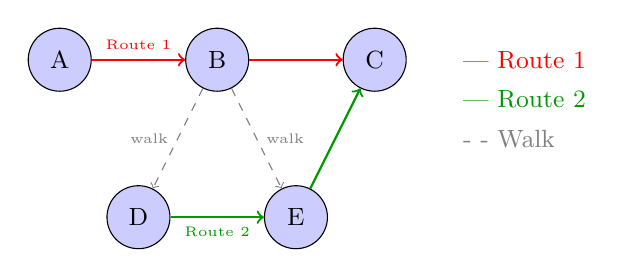
\begin{tikzpicture}[
        stop/.style={circle, draw, fill=blue!20, minimum size=0.8cm, font=\small},
        route1/.style={->, thick, red},
        route2/.style={->, thick, green!60!black},
        walk/.style={->, dashed, gray}
    ]
        % Stops
        \node[stop] (A) at (0, 2) {A};
        \node[stop] (B) at (2, 2) {B};
        \node[stop] (C) at (4, 2) {C};
        \node[stop] (D) at (1, 0) {D};
        \node[stop] (E) at (3, 0) {E};
        
        % Route 1 (red)
        \draw[route1] (A) -- node[above] {\tiny Route 1} (B);
        \draw[route1] (B) -- (C);
        
        % Route 2 (green)
        \draw[route2] (D) -- node[below] {\tiny Route 2} (E);
        \draw[route2] (E) -- (C);
        
        % Walking edges (dashed)
        \draw[walk] (B) -- node[left] {\tiny walk} (D);
        \draw[walk] (B) -- node[right] {\tiny walk} (E);
        
        % Legend
        \node[right] at (5, 2) {\small \textcolor{red}{--- Route 1}};
        \node[right] at (5, 1.5) {\small \textcolor{green!60!black}{--- Route 2}};
        \node[right] at (5, 1) {\small \textcolor{gray}{- - Walk}};
    \end{tikzpicture}
    \caption{Graph Abstraction of Bus Network with Walking Transfers}
    \label{fig:graph-abstraction}
\end{figure}

\textbf{Key insight:} By representing transfers as walking edges, the A* algorithm can seamlessly find multi-route journeys without special transfer logic.

\subsection{Procedural Abstraction: API Interfaces}

Procedural abstraction hides implementation complexity behind clean function interfaces.

\paragraph{Example: Route Finding Abstraction}

\begin{lstlisting}[language=Python, caption={Procedural Abstraction - Clean API Interface}]
# What the API endpoint exposes (abstracted interface)
@app.route('/api/bus/route')
def get_bus_route():
    """
    Abstraction: Complex pathfinding -> Simple request/response
    
    User only needs to know:
    - Input: origin (lat, lng), destination (lat, lng)
    - Output: route with stops, buses, fare, duration
    
    Hidden complexity:
    - Graph loading and caching
    - A* algorithm implementation
    - Transfer penalty calculations
    - Walking distance computations
    - Fare calculation logic
    """
    origin = (request.args.get('origin_lat'), request.args.get('origin_lng'))
    dest = (request.args.get('dest_lat'), request.args.get('dest_lng'))
    
    # All complexity hidden behind this single function call
    route = find_optimal_route(origin, dest)
    
    return jsonify(route)

# Implementation details hidden from API users
def find_optimal_route(origin, dest):
    G = get_cached_graph()           # Hidden: caching logic
    start_stops = nearby_stops(origin)  # Hidden: haversine calculations
    end_stops = nearby_stops(dest)
    path = a_star(G, start_stops, end_stops)  # Hidden: algorithm details
    return format_route_response(path)  # Hidden: data transformation
\end{lstlisting}

\paragraph{Abstraction Layers in the System}

\begin{table}[H]
    \centering
    \renewcommand{\arraystretch}{1.2}
    \begin{tabularx}{\textwidth}{|l|X|X|}
        \hline
        \textbf{Layer} & \textbf{What it Exposes} & \textbf{What it Hides} \\
        \hline
        REST API & HTTP endpoints with JSON I/O & Flask internals, database queries, algorithm logic \\
        \hline
        Service Layer & \texttt{find\_route()}, \texttt{detect\_vehicles()} & Graph operations, YOLO inference, caching \\
        \hline
        Data Layer & \texttt{get\_stops()}, \texttt{get\_cameras()} & SQL queries, CSV parsing, file I/O \\
        \hline
        Algorithm Layer & \texttt{a\_star()}, \texttt{haversine()} & Priority queue, math operations, edge traversal \\
        \hline
    \end{tabularx}
    \caption{Procedural Abstraction Layers}
\end{table}

\subsection{Benefits of Abstraction in This Project}

\paragraph{1. Reduced Complexity}
Without abstraction, the bus routing function would need to handle:
\begin{itemize}[noitemsep]
    \item Raw CSV parsing for 4,343 stops
    \item Complex SQL joins for route-stop relationships
    \item Manual distance calculations for every stop pair
    \item Direct graph traversal with priority queue management
\end{itemize}
With abstraction, it becomes a single function call: \texttt{find\_optimal\_route(origin, dest)}

\paragraph{2. Improved Maintainability}
\begin{lstlisting}[language=Python, caption={Abstraction Enables Easy Updates}]
# If we need to change distance calculation (e.g., add elevation):
# Only modify ONE function, not 50+ call sites

def haversine(c1, c2):
    # Original: spherical distance only
    # Updated: can add elevation factor here
    base_distance = calculate_spherical_distance(c1, c2)
    elevation_factor = get_elevation_adjustment(c1, c2)
    return base_distance * elevation_factor
\end{lstlisting}

\paragraph{3. Enabled Testing}
Abstraction allows testing components in isolation:
\begin{lstlisting}[language=Python, caption={Abstraction Enables Unit Testing}]
class TestBusRouting(unittest.TestCase):
    def test_haversine_accuracy(self):
        # Test distance function independently
        dist = haversine((10.7769, 106.7009), (10.8231, 106.6297))
        self.assertAlmostEqual(dist, 8900, delta=100)  # ~8.9km
    
    def test_nearby_stops(self):
        # Test stop finding independently
        stops = nearby_stops(10.7769, 106.7009, radius=500)
        self.assertTrue(len(stops) > 0)
\end{lstlisting}

\paragraph{4. Facilitated Team Collaboration}
Each team member could work on their module independently:
\begin{itemize}[noitemsep]
    \item \textbf{Database team:} Implement data layer, expose \texttt{get\_stops()}
    \item \textbf{Algorithm team:} Implement \texttt{a\_star()}, assume graph exists
    \item \textbf{API team:} Build endpoints, call service functions
    \item \textbf{Frontend team:} Consume REST API, ignore backend complexity
\end{itemize}

\subsection{Abstraction Trade-offs}

While abstraction provides many benefits, we also considered its limitations:

\begin{table}[H]
    \centering
    \renewcommand{\arraystretch}{1.2}
    \begin{tabularx}{\textwidth}{|X|X|}
        \hline
        \textbf{Benefit} & \textbf{Trade-off} \\
        \hline
        Simplified bus stop data (5 attributes) & Cannot provide accessibility infomation without re-adding attributes \\
        \hline
        Aggregate vehicle counts & Cannot track individual vehicles or measure speeds \\
        \hline
        Graph abstraction of bus network & Loses real-time schedule information \\
        \hline
        Hidden algorithm complexity & Harder to debug when issues occur deep in the stack \\
        \hline
    \end{tabularx}
    \caption{Abstraction Trade-offs Considered}
\end{table}

\textbf{Design Decision:} We prioritized simplicity for the MVP (Minimum Viable Product). Additional attributes can be added later without changing the core architecture.

\section{Algorithm Design}

Algorithm design is the fourth pillar of computational thinking, transforming our decomposed problems, recognized patterns, and abstractions into step-by-step procedures that can be executed by computers. This section details the key algorithms developed for this project.

\subsection{Overview of Algorithmic Approaches}

\begin{table}[H]
    \centering
    \renewcommand{\arraystretch}{1.3}
    \begin{tabularx}{\textwidth}{|l|l|X|}
        \hline
        \textbf{Algorithm} & \textbf{Paradigm} & \textbf{Application} \\
        \hline
        A* Search & Graph Search & Optimal bus route finding \\
        \hline
        Percentile Threshold & Statistical & Traffic congestion classification \\
        \hline
        YOLO Detection & Deep Learning & Vehicle counting from camera images \\
        \hline
        Fuzzy String Matching & Approximate Matching & Place name resolution \\
        \hline
        LLM Prompting & AI/NLP & Trip itinerary generation \\
        \hline
        Haversine Distance & Computational Geometry & GPS distance calculations \\
        \hline
    \end{tabularx}
    \caption{Algorithmic Approaches Used in the Project}
\end{table}

\subsection{System Architecture Flowchart}

\begin{figure}[H]
    \centering
    \begin{tikzpicture}[
        node distance=1.5cm,
        box/.style={rectangle, draw, minimum width=2.5cm, minimum height=0.9cm, align=center, font=\small},
        db/.style={cylinder, draw, shape border rotate=90, aspect=0.25, minimum height=1cm, minimum width=1.5cm, font=\small},
        arrow/.style={->, thick}
    ]
        % User Request
        \node[box, fill=gray!20] (user) {User Request\\(Web/Mobile)};
        
        % API Layer
        \node[box, fill=blue!20, below=of user] (api) {Flask API\\Server};
        
        % Endpoints
        \node[box, fill=green!15, below left=1.2cm and 5cm of api] (auth) {/api/auth/*};
        \node[box, fill=green!15, below left=1.2cm and 1cm of api] (route) {/route};
        \node[box, fill=green!15, below=1.2cm of api] (bus) {/api/bus/route};
        \node[box, fill=green!15, below right=1.2cm and 1cm of api] (groq) {/api/groq};
        
        % Services
        \node[db, fill=yellow!30, below=of auth] (mysql) {MySQL};
        \node[box, fill=orange!20, below=of route] (tomtom) {TomTom\\API};
        \node[box, fill=purple!20, below=of bus] (astar) {A*\\Algorithm};
        \node[box, fill=red!20, below=of groq] (llm) {Groq\\LLM};
        
        % Traffic Detection
        \node[box, fill=pink!20, below right=1.2cm and 4cm of api] (yolo) {YOLO v11\\Vehicle Detection};



        % Arrows
        \draw[arrow] (user) -- (api);
        \draw[arrow] (api) -- (auth);
        \draw[arrow] (api) -- (route);
        \draw[arrow] (api) -- (bus);
        \draw[arrow] (api) -- (groq);
        \draw[arrow] (auth) -- (mysql);
        \draw[arrow] (route) -- (tomtom);
        \draw[arrow] (bus) -- (astar);
        \draw[arrow] (api) -- (yolo);
        \draw[arrow] (groq) -- (llm);
    \end{tikzpicture}
    \caption{System Architecture Flowchart}
    \label{fig:system-arch}
\end{figure}

% ============================================
% ALGORITHM 1: A* BUS ROUTING
% ============================================
\subsection{Algorithm 1: A* Bus Routing}

\paragraph{Problem Statement}
Given a user's origin and destination coordinates, find the optimal bus route minimizing travel time, transfer penalties, and fare costs.

\paragraph{Why A*?}
A* combines Dijkstra's optimality guarantee with heuristic guidance, making it faster than Dijkstra while still finding the optimal path. Our admissible heuristic never overestimates, ensuring optimality.

\paragraph{Key Design Decision}
States are represented as \textbf{(stop, current\_route)} pairs, not just stops. This allows tracking transfer costs when changing routes at the same physical stop.

\paragraph{Cost Function}
\begin{equation}
    g(u \rightarrow v) = \frac{d_{uv}}{v_{\text{mode}}} + P_{\text{transfer}} \cdot \mathbb{1}_{\text{transfer}} + C_{\text{fare}} \cdot f_{uv} \cdot \mathbb{1}_{\text{new\_route}}
\end{equation}

Parameters: $P_{\text{transfer}} = 10.0$, $C_{\text{fare}} = 5.0$.
\[
v_{\text{mode}} =
\begin{cases}
    7 & \text{m/s (bus edge)}\\
    1.5 & \text{m/s (walk edge)}
\end{cases}
\]

Where: 
\begin{itemize}[noitemsep]
    \item $v_{\text{mode}}$ = speed based on edge mode
    \item $P_{\text{transfer}}$ = maximum time penalty for transfers
    \item $d_{uv}$ = distance between stops $u$ and $v$
    \item $\mathbb{1}_{\text{transfer}}$ = 1 if changing routes, else 0
    \item $f_{uv}$ = fare tranfer $u \rightarrow v$
    \item $\mathbb{1}_{\text{new\_route}}$ = 1 if boarding a new route, else 0
\end{itemize}

\paragraph{Pseudocode}

\begin{algorithm}[H]
\caption{A* Bus Routing}
\begin{algorithmic}[1]
\REQUIRE origin coordinates, destination coordinates
\ENSURE optimal bus route with minimal cost
\STATE nearby\_starts $\gets$ find\_stops\_within(origin, MAX\_WALK\_DIST)
\STATE nearby\_goals $\gets$ find\_stops\_within(destination, MAX\_WALK\_DIST)
\STATE open\_set $\gets$ PriorityQueue()
\FOR{each stop in nearby\_starts}
    \STATE open\_set.push((stop, ``walk''), f=h(stop))
\ENDFOR
\STATE g\_score $\gets$ \{\}, came\_from $\gets$ \{\}
\WHILE{open\_set not empty}
    \STATE current $\gets$ open\_set.pop\_min()
    \IF{current.stop in nearby\_goals}
        \RETURN reconstruct\_path(came\_from, current)
    \ENDIF
    \FOR{each neighbor in get\_neighbors(current)}
        \STATE cost $\gets$ travel\_time + transfer\_penalty + fare\_cost
        \STATE tentative\_g $\gets$ g\_score[current] + cost
        \IF{tentative\_g $<$ g\_score[neighbor]}
            \STATE g\_score[neighbor] $\gets$ tentative\_g
            \STATE came\_from[neighbor] $\gets$ current
            \STATE f $\gets$ tentative\_g + h(neighbor)
            \STATE open\_set.push(neighbor, f)
        \ENDIF
    \ENDFOR
\ENDWHILE
\RETURN no\_route\_found
\end{algorithmic}
\end{algorithm}

\paragraph{Complexity}
\begin{itemize}[noitemsep]
    \item \textbf{Time:} $O((V \cdot R) \log (V \cdot R))$ where $V$ = stops, $R$ = routes
    \item \textbf{Space:} $O(V \cdot R)$ for state space
    \item \textbf{Practical:} 50-200ms for HCMC queries (4,343 stops, 127 routes)
\end{itemize}

% ============================================
% ALGORITHM 2: YOLO VEHICLE DETECTION
% ============================================
\subsection{Algorithm 2: YOLO Vehicle Detection}

\paragraph{Problem Statement}
Given a traffic camera image, count vehicles by type (car, motorcycle, bus, truck) to estimate traffic density.

\paragraph{Why YOLO v11?}
YOLO provides real-time object detection with high accuracy, making it ideal for processing traffic camera feeds. Unlike two-stage detectors like Faster R-CNN, YOLO processes the entire image in a single forward pass.

\paragraph{Detection Pipeline}

\begin{figure}[H]
    \centering
    \begin{tikzpicture}[
        node distance=0.6cm,
        box/.style={rectangle, draw, minimum width=2cm, minimum height=1cm, align=center, font=\small},
        arrow/.style={->, thick}
    ]
        \node[box, fill=gray!20] (input) {Camera\\Image};
        \node[box, fill=blue!20, right=of input] (clahe) {CLAHE};
        \node[box, fill=green!20, right=of clahe] (yolo) {YOLO v11};
        \node[box, fill=orange!20, right=of yolo] (filter) {Filter};
        \node[box, fill=purple!20, right=of filter] (count) {Counts};
        
        \draw[arrow] (input) -- (clahe);
        \draw[arrow] (clahe) -- (yolo);
        \draw[arrow] (yolo) -- (filter);
        \draw[arrow] (filter) -- (count);
    \end{tikzpicture}
    \caption{Vehicle Detection Pipeline}
\end{figure}

\paragraph{Pseudocode}

\begin{algorithm}[H]
\caption{YOLO Vehicle Detection}
\begin{algorithmic}[1]
\REQUIRE camera\_image (960$\times$540)
\ENSURE vehicle\_counts dictionary
\STATE \textit{// Preprocessing: enhance low-light images}
\STATE lab $\gets$ convert\_to\_LAB(camera\_image)
\STATE lab.L $\gets$ apply\_CLAHE(lab.L, clip\_limit=2.0, grid=8×8)
\STATE enhanced $\gets$ convert\_to\_RGB(lab)
\STATE \textit{// Run YOLO inference}
\STATE detections $\gets$ yolo\_model.predict(enhanced, conf=0.15)
\STATE \textit{// Filter by class-specific thresholds}
\STATE THRESHOLDS $\gets$ \{motorcycle: 0.15, car: 0.25, truck: 0.30, bus: 0.38\}
\STATE counts $\gets$ \{motorcycle: 0, car: 0, truck: 0, bus: 0\}
\FOR{each detection in detections}
    \IF{detection.confidence $\geq$ THRESHOLDS[detection.class]}
        \STATE counts[detection.class] += 1
    \ENDIF
\ENDFOR
\RETURN counts
\end{algorithmic}
\end{algorithm}

\paragraph{Key Implementation Details}
\begin{itemize}[noitemsep]
    \item \textbf{CLAHE Preprocessing:} Enhances contrast in poor lighting conditions by operating on the L channel of LAB color space
    \item \textbf{Class-Specific Thresholds:} Motorcycles (small, often occluded) use lower threshold (0.15); buses (large, distinctive) use higher threshold (0.38)
\end{itemize}

% ============================================
% ALGORITHM 3: CONGESTION CLASSIFICATION
% ============================================
\subsection{Algorithm 3: Percentile-Based Congestion Classification}

\paragraph{Problem Statement}
Given a vehicle count for a road segment, classify traffic as ``green'' (free flow), ``yellow'' (moderate), or ``red'' (congested).

\paragraph{Why Percentile Thresholds?}
Fixed thresholds don't work across different road types---a highway with 50 vehicles is normal, but a residential street with 50 vehicles is severely congested. Percentile-based thresholds adapt to each segment's historical traffic patterns.

\paragraph{Classification Logic}

\begin{figure}[H]
    \centering
    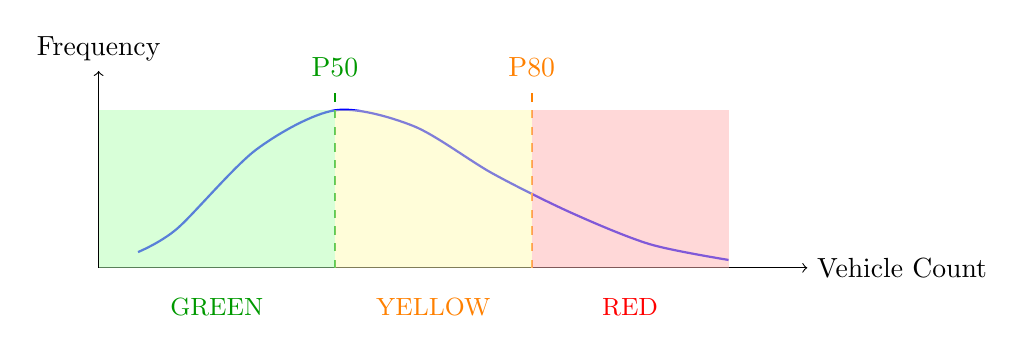
\begin{tikzpicture}
        % Axis
        \draw[->] (0,0) -- (9,0) node[right] {Vehicle Count};
        \draw[->] (0,0) -- (0,2.5) node[above] {Frequency};
        
        % Distribution curve
        \draw[thick, blue] plot[smooth] coordinates {(0.5,0.2) (1,0.5) (2,1.5) (3,2) (4,1.8) (5,1.2) (6,0.7) (7,0.3) (8,0.1)};
        
        % Threshold lines
        \draw[dashed, green!60!black, thick] (3,0) -- (3,2.3) node[above] {P50};
        \draw[dashed, orange, thick] (5.5,0) -- (5.5,2.3) node[above] {P80};
        
        % Colored regions
        \fill[green!30, opacity=0.5] (0,0) rectangle (3,2);
        \fill[yellow!30, opacity=0.5] (3,0) rectangle (5.5,2);
        \fill[red!30, opacity=0.5] (5.5,0) rectangle (8,2);
        
        % Labels
        \node[font=\small, green!60!black] at (1.5, -0.5) {GREEN};
        \node[font=\small, orange] at (4.25, -0.5) {YELLOW};
        \node[font=\small, red] at (6.75, -0.5) {RED};
    \end{tikzpicture}
    \caption{Percentile-Based Classification}
\end{figure}

\paragraph{Pseudocode}

\begin{algorithm}[H]
\caption{Congestion Classification}
\begin{algorithmic}[1]
\REQUIRE segment\_id, vehicle\_count
\ENSURE congestion\_level $\in$ \{green, yellow, red\}
\STATE thresholds $\gets$ load\_thresholds(segment\_id)
\IF{thresholds not found}
    \STATE thresholds $\gets$ calculate\_from\_history(segment\_id)
    \IF{insufficient data}
        \STATE thresholds $\gets$ DEFAULT\_THRESHOLDS
    \ENDIF
\ENDIF
\STATE P50, P80 $\gets$ thresholds
\IF{vehicle\_count $\leq$ P50}
    \RETURN ``green'' \COMMENT{Free flow: below median}
\ELSIF{vehicle\_count $\leq$ P80}
    \RETURN ``yellow'' \COMMENT{Moderate: 50th-80th percentile}
\ELSE
    \RETURN ``red'' \COMMENT{Congested: above 80th percentile}
\ENDIF
\end{algorithmic}
\end{algorithm}

\paragraph{Threshold Calculation}
Thresholds are pre-computed from historical data and stored in \texttt{segment\_thresholds.json}:
\begin{itemize}[noitemsep]
    \item \textbf{P50} (median): 50\% of historical observations fall below this value
    \item \textbf{P80}: 80\% of historical observations fall below this value
    \item \textbf{Fallback}: For new segments with insufficient data, use city-wide defaults
\end{itemize}

% ============================================
% ALGORITHM 4: AI TRIP PLANNING
% ============================================
\newpage
\subsection{Algorithm 4: AI Trip Planning with Fuzzy Matching}

\paragraph{Problem Statement}
Given a natural language query (e.g., ``Plan a day trip visiting museums and cafes''), generate an optimized itinerary with real coordinates and routes.

\paragraph{Three-Stage Pipeline}

\begin{figure}[H]
    \centering
    \begin{tikzpicture}[
        node distance=1.5cm,
        box/.style={rectangle, draw, rounded corners, minimum width=2.2cm, minimum height=1cm, align=center, font=\small},
        arrow/.style={->, thick}
    ]
        \node[box, fill=gray!20] (input) {User Query};
        \node[box, fill=red!20, right=of input] (llm) {Groq LLM};
        \node[box, fill=blue!20, right=of llm] (fuzzy) {RapidFuzz};
        \node[box, fill=green!20, right=of fuzzy] (routing) {TomTom API};
        \node[box, fill=purple!20, right=of routing] (output) {Itinerary};
        
        \draw[arrow] (input) -- (llm);
        \draw[arrow] (llm) -- node[above, font=\tiny] {place names} (fuzzy);
        \draw[arrow] (fuzzy) -- node[above, font=\tiny] {coordinates} (routing);
        \draw[arrow] (routing) -- (output);
    \end{tikzpicture}
    \caption{AI Trip Planning Pipeline}
\end{figure}

\paragraph{Fallback Mechanisms}

\definecolor{aiRed}{HTML}{FFCDD2}
\definecolor{aiBorder}{HTML}{D32F2F}
\definecolor{procBlue}{HTML}{E1F5FE}
\definecolor{procBorder}{HTML}{0288D1}
\definecolor{dbYellow}{HTML}{FFF9C4}
\definecolor{dbBorder}{HTML}{FBC02D}
\definecolor{fallbackOrange}{HTML}{FFE0B2}
\definecolor{fallbackBorder}{HTML}{F57C00}
\definecolor{routeGreen}{HTML}{C8E6C9}
\definecolor{routeBorder}{HTML}{388E3C}


\begin{figure}[H]
    \centering
\begin{tikzpicture}[
    node distance=1.5cm and 1.5cm,
    % Styles
    base/.style={
        draw, 
        align=center, 
        font=\sffamily\small,
        line width=0.8pt
    },
    process/.style={
        base, 
        rectangle, 
        rounded corners=3pt, 
        fill=procBlue, 
        draw=procBorder, 
        minimum width=2.5cm, 
        minimum height=1cm
    },
    llm/.style={
        base, 
        rectangle, 
        rounded corners=3pt, 
        fill=red!20, 
        draw=aiBorder, 
        minimum width=2.5cm, 
        minimum height=1cm
    },
    database/.style={
        base,
        cylinder, 
        shape border rotate=90, 
        aspect=0.25, 
        fill=dbYellow, 
        draw=dbBorder, 
        minimum width=2cm, 
        minimum height=1.5cm
    },
    fallback/.style={
        base, 
        rectangle, 
        dashed,
        rounded corners=3pt, 
        fill=fallbackOrange, 
        draw=fallbackBorder, 
        minimum width=2.5cm, 
        minimum height=1cm
    },
    routing/.style={
        base, 
        rectangle, 
        rounded corners=3pt, 
        fill=green!20, 
        draw=routeBorder, 
        minimum width=2.5cm, 
        minimum height=1cm
    },
    connector/.style={
        -Latex, 
        thick, 
        draw=black!70,
        rounded corners
    },
    labeltext/.style={
        font=\sffamily\tiny, 
        midway, 
        fill=white, 
        text=black!70, 
        inner sep=1.5pt,
        rounded corners=2pt
    }
]

    % --- Nodes ---
    
    % 1. Input/Generation
    \node[llm] (groq) {Groq LLM};
    
    % 2. Fuzzy Match (The "Fuzzy" node in sketch)
    \node[process, right=of groq] (fuzzy) {RapidFuzz\\Verification};
    
    % 3. Database (The "Data base" node in sketch)
    \node[database, right=of fuzzy] (db) {Location\\Database};
    
    % 4. Fallback (The "GeoApify/OSM" node in sketch)
    % Positioned below to represent the "Fail" path
    \node[fallback, below=1.5cm of fuzzy] (geocoder) {GeoApify / OSM\\(External Geocode)};
    
    % 5. Routing (The "Tom Tom" node in sketch)
    \node[routing, right=of db] (tomtom) {TomTom\\Route Calc};

    % --- Connections ---

    % Flow: LLM -> Fuzzy
    \draw[connector] (groq) -- node[labeltext] {Place Names} (fuzzy);

    % Path A: Success (Fuzzy -> DB)
    \draw[connector] (fuzzy) -- node[labeltext, text=green!60!black] {Match Found} (db);

    % Path B: Failure (Fuzzy -> Fail -> GeoApify)
    \draw[connector, red] (fuzzy.south) -- node[labeltext, text=red] {Fail / No Match} (geocoder.north);

    % Path B return: GeoApify -> DB 
    % (Sketch shows arrow pointing from GeoApify to Database)
    \draw[connector, dashed] (geocoder.east) -| node[labeltext, pos=0.2] {New Coords} (db.south);

    % Final Flow: DB -> Routing
    \draw[connector] (db) -- node[labeltext] {Lat / Lng} (tomtom);

\end{tikzpicture}
\end{figure}



\paragraph{Pseudocode}

\begin{algorithm}[H]
\caption{AI Trip Planning}
\begin{algorithmic}[1]
\REQUIRE user\_query, database
\ENSURE trip\_plan (JSON with coordinates and routes)

\STATE \textit{// Stage 1: LLM Generates Structured Itinerary}
\STATE prompt $\gets$ build\_prompt(user\_query, "HCMC Context")
\STATE raw\_json $\gets$ groq\_api.generate(prompt, model="llama-3.3-70b")
\STATE itinerary $\gets$  parse\_json(raw\_json)

\STATE \textit{// Stage 2: Resolution \& Fallback Logic}
\FORALL{place \textbf{in} itinerary}
    \STATE match $\gets$ rapidfuzz.extract(place.name, database)
    
    \IF{match.score $\geq$ THRESHOLD}
        \STATE \textit{// Case A: Found in Verified Database}
        \STATE place.coords $\gets$ match.coords
        \STATE place.image $\gets$ match.image\_path
        \STATE place.matched $\gets$ \textbf{true}
    \ELSE
        \STATE \textit{// Case B: Fallback to External Geocoding}
        \STATE geo\_result $\gets$ geocode\_api.geocode(place.address)
        \IF{geo\_result $\neq$ null}
            \STATE place.coords $\gets$ geo\_result.coords
        \ENDIF
        \STATE place.image $\gets$ generic\_image\_match(place.type)
        \STATE place.matched $\gets$ \textbf{false}
    \ENDIF
\ENDFOR

\STATE \textit{// Stage 3: Routing Calculation}
\STATE routes $\gets$ []
\FOR{i $\gets$ 0 \textbf{to} length(itinerary) - 2}
    \IF{itinerary[i] has coords \textbf{and} itinerary[i+1] has coords}
        \STATE segment $\gets$ tomtom\_api.route(itinerary[i], itinerary[i+1])
        \STATE routes.append(segment)
    \ENDIF
\ENDFOR

\RETURN \{ plan: itinerary, routes: routes \}
\end{algorithmic}
\end{algorithm}

\paragraph{Key Components}
\begin{itemize}[noitemsep]
    \item \textbf{Groq LLM:} Generates itineraries with place names, times, and descriptions (1-2s)
    \item \textbf{RapidFuzz:} Matches LLM output (``Ben Thanh Market'') to database entries (``Chợ Bến Thành'') with 70\% minimum similarity threshold
    \item \textbf{TomTom API:} Calculates optimal driving routes and travel times between consecutive stops
\end{itemize}

% ============================================
% ALGORITHM 5: HAVERSINE DISTANCE
% ============================================
\subsection{Algorithm 5: Haversine Distance Calculation}

\paragraph{Problem Statement}
Calculate the great-circle distance between two GPS coordinates, accounting for Earth's curvature.

\paragraph{Why Not Euclidean Distance?}
Euclidean distance treats coordinates as flat 2D points, which introduces significant error over larger distances. Haversine calculates the shortest path along Earth's curved surface.

\paragraph{The Haversine Formula}

\begin{equation}
    a = \sin^2\left(\frac{\Delta\phi}{2}\right) + \cos(\phi_1) \cdot \cos(\phi_2) \cdot \sin^2\left(\frac{\Delta\lambda}{2}\right)
\end{equation}
\begin{equation}
    d = 2R \cdot \arctan2\left(\sqrt{a}, \sqrt{1-a}\right)
\end{equation}

Where: $\phi$ = latitude (radians), $\lambda$ = longitude (radians), $R$ = 6,371 km

\paragraph{Pseudocode}

\begin{algorithm}[H]
\caption{Haversine Distance}
\begin{algorithmic}[1]
\REQUIRE lat1, lon1, lat2, lon2 (in degrees)
\ENSURE distance in meters
\STATE R $\gets$ 6,371,000 \COMMENT{Earth's radius in meters}
\STATE $\phi_1$ $\gets$ radians(lat1), $\phi_2$ $\gets$ radians(lat2)
\STATE $\Delta\phi$ $\gets$ radians(lat2 - lat1)
\STATE $\Delta\lambda$ $\gets$ radians(lon2 - lon1)
\STATE a $\gets$ $\sin^2(\Delta\phi/2) + \cos(\phi_1) \cdot \cos(\phi_2) \cdot \sin^2(\Delta\lambda/2)$
\STATE c $\gets$ $2 \cdot \text{atan2}(\sqrt{a}, \sqrt{1-a})$
\RETURN R $\times$ c
\end{algorithmic}
\end{algorithm}

\paragraph{Usage Across the Project}
The haversine function is a \textbf{core utility} reused 50+ times across:
\begin{itemize}[noitemsep]
    \item \textbf{Bus Routing:} Finding nearby stops within walking distance
    \item \textbf{Graph Builder:} Calculating edge distances between stops
    \item \textbf{API Filters:} Location-based camera and place queries
    \item \textbf{Segment Matching:} Associating cameras with road segments
    \item \textbf{Trip Planning:} Checking place proximity
\end{itemize}

\subsection{Algorithm Design Summary}

\begin{table}[H]
    \centering
    \renewcommand{\arraystretch}{1.3}
    \begin{tabularx}{\textwidth}{|l|l|l|X|}
        \hline
        \textbf{Algorithm} & \textbf{Complexity} & \textbf{Performance} & \textbf{Key Insight} \\
        \hline
        A* Routing & $O(VR \log VR)$ & 50-200ms & State = (stop, route) enables transfer penalties \\
        \hline
        YOLO Detection & $O(HW)$ & 100-500ms & Class-specific thresholds improve accuracy \\
        \hline
        Congestion & $O(1)$ & $<$1ms & Percentile thresholds adapt to each segment \\
        \hline
        Trip Planning & $O(N^2)$ & 2-5s & Fuzzy matching bridges LLM and database \\
        \hline
        Haversine & $O(1)$ & $<$0.1ms & Reused 50+ times across modules \\
        \hline
    \end{tabularx}
    \caption{Algorithm Performance Summary}
\end{table}

